\documentclass{article}

% Packages
\usepackage{geometry}
\usepackage{graphicx}
\usepackage{lipsum}
\usepackage{listings}
\usepackage[portuguese]{babel}

% -- Defining colors:
\usepackage[dvipsnames]{xcolor}
\definecolor{codegreen}{rgb}{0,0.6,0}
\definecolor{codegray}{rgb}{0.5,0.5,0.5}
\definecolor{codepurple}{rgb}{0.58,0,0.82}
\definecolor{backcolour}{rgb}{0.95,0.95,0.92}

% Definig a custom style:
\lstdefinestyle{mystyle}{
    backgroundcolor=\color{backcolour},   
    commentstyle=\color{codepurple},
    keywordstyle=\color{NavyBlue},
    numberstyle=\tiny\color{codegray},
    stringstyle=\color{codepurple},
    basicstyle=\ttfamily\footnotesize\bfseries,
    breakatwhitespace=false,
    breaklines=true,
    keepspaces=true,
    numbers=left,
    numbersep=5pt,
    showspaces=false,
    showstringspaces=false,
    showtabs=false,
    tabsize=2,
    captionpos=b
}

% -- Setting up the custom style:
\lstset{style=mystyle}

% Page setup
\geometry{a4paper, margin=2cm}

\begin{document}

% cover
\thispagestyle{empty} % Remove page number from first page

\begin{figure}[t]
    
\includegraphics[width=3cm]{images/logo-puc-minas.png}
    \hspace{0.02\textwidth}
    \vline%
    \hspace{0.04\textwidth}
    
\includegraphics[width=3cm]{images/logo-icei.jpeg}
\end{figure}

\hrulefill%
\vspace{\baselineskip}

\Large\noindent
\textbf{Pontifícia Universidade Católica de Minas Gerais} \\
\textbf{Instituto de Ciências Exatas e Informática} \\
\textbf{Departamento de Engenharia de Computação}

\begin{center}
    \vfill
    \Huge\textbf{Relatório: Trabalho Prático 2} \\
    \vspace{0.5cm}
    \Large\textbf{Registradores em VHDL} \\
    \vspace{1cm}
    \large \textbf{Professor(es)}: Antônio Hamilton Magalhães\\
    \vspace{0.5cm}
    \large \textbf{Aluno(s)}: Bruno Luiz Dias Alves de Castro \\
    \large \hspace{0.75cm} Rafael Ramos de Andrade \\
    \vfill
    \large Belo Horizonte \\ Campus Coração Eucarístico \\
    \vspace{\baselineskip}
    \large \today
\end{center}

% table of contents
\newpage
\thispagestyle{empty}
\tableofcontents

% body
\newpage
\large % document text size

\section{Introdução}

Durante as aulas da disciplina de Sistemas Reconfiguráveis, fomos introduzidos à linguagem VHDL. VHDL (\textbf{V}HSIC \textbf{H}ardware \textbf{D}escription \textbf{L}anguage) é uma linguagem de descrição de hardware. Com ela, podemos montar circuitos lógicos de maneira totalmente textual, o que garante à linguagem uma grande vantagem ante à soluções visuais.

\subsection{Objetivos}

O objetivo deste terceiro trabalho prático é a implementação de uma memória ram e uma porta com barramento bidirecional. Essas estruturas serão utilizadas na construção interna do processador e para interfacear a comunicação interna e externa, respectivamente. Uma breve descrição de cada um é apresentada à seguir:

\subsubsection{port\_io}

O bloco port\_io é utilizado na comunicação entre a parte interna e externa do processador. É constituído de um barramento bidirecional configurado por um registrador nomeado tris\_reg, que define quais sinais serão entrada e saída.

\subsubsection{ram\_mem}

O bloco de ram\_mem, ou memória ram, são 4 registradores de propósito geral acessados através de endereços configurados na porta de endereçamento. Cada registrador é acessado por uma faixa de endereços, suportam acesso para escrita ou leitura.

\newpage

\section{port\_io}

O port\_io  é um circuito que possui uma estrutura de dois registradores de 8 bits, e um barramento bidirecional de entrada e saída, para interfaceamento com a estrutura. O registrador tris\_reg armazena o estado de cada bit (que pode ser entrada e saída), e o registrador port\_reg armazena dados, que podem ser escritos pelo usuário através do barramento de dados dbus\_in.

As entradas e saídas do circuito são descritas na tabela abaixo:\\

\begin{table}[ht]
    \begin{center}
        \begin{tabular}{|c|c|c|c|}
            \hline
            Nome & Tamanho & Tipo & Descrição\\
            \hline
            nrst & 1 bit & \textit{Input} & Entrada de \textit{reset} assíncrono.\\
            \hline
            clk\_in & 1 bit & \textit{Input} & Entrada de \textit{clock}.\\
            \hline
            abus\_in & 9 bits & \textit{Input} & Entrada de endereçamento para os registradores internos.\\
            \hline
            dbus\_in & 8 bits & \textit{Input} & Entrada de habilitação para escrita nos registradores\\
            \hline
            wr\_en & 1 bit & \textit{Input} & Entrada de habilitação de escrita.\\
            \hline
            rd\_en & 1 bit & \textit{Input} & Entrada de habilitação de leitura.\\
            \hline
            dbus\_out & 8 bits & \textit{Output} & Barramento de saída de dados, com 8 bits.\\
            \hline
            port\_io & 8 bits & \textit{Inout} & Porta bidirecional, com 8 bits.\\
            \hline
        \end{tabular}
    \end{center}
    \caption{Entradas e Saídas de port\_io}
\end{table}

Para o port\_io, também são utilizados 4 endereços internos, implementados através de estruturas \textit{GENERIC}, para endereçamento dos registradores tris\_reg e port\_reg. São eles:

\begin{table}[ht]
\begin{center}
\begin{tabular}{|c|c|c|}
    \hline
    Nome & Endereço & Descrição \\
    \hline
    port\_addr & 0b00000011 & Especifica o endereço de escrita no registrador port\_reg. \\
    \hline
    tris\_addr & 0b00000111 & Especifica o endereço de escrita no registrador tris\_reg. \\
    \hline
    alt\_port\_addr & 0b10000000 & Endereço alternativo a port\_addr. \\
    \hline
    alt\_tris\_addr & 0b11000000 & Endereço alternativo a tris\_addr. \\
    \hline
\end{tabular}
\end{center}
\end{table}

\subsection{Implementação}

O circuito port\_io foi implementado utilizando a linguagem VHDL.\\

O código na íntegra está abaixo:\\

\begin{lstlisting}[language=VHDL, caption={Código VHDL w\_reg}]
LIBRARY ieee;
USE ieee.std_logic_1164.all;
USE ieee.std_logic_unsigned.all;
USE ieee.numeric_std.all;

ENTITY port_io IS
    GENERIC (
        -- enderecos dos registradores port a tris
        port_addr: IN STD_LOGIC_VECTOR(8 DOWNTO 0) :=  "000000011";
        tris_addr: IN STD_LOGIC_VECTOR(8 DOWNTO 0) :=  "000000111";
        alt_port_addr: IN STD_LOGIC_VECTOR(8 DOWNTO 0) :=  "100000000";
        alt_tris_addr: IN STD_LOGIC_VECTOR(8 DOWNTO 0) :=  "110000000"
    );
    PORT (
        -- Processor Side
        -- Inputs
        nrst : IN STD_LOGIC;                            -- Reset
        clk_in: IN STD_LOGIC;                           -- Clock
        abus_in: IN STD_LOGIC_VECTOR(8 DOWNTO 0);       -- Enderecamento
        dbus_in: IN STD_LOGIC_VECTOR(7 DOWNTO 0);       -- Dados
        wr_en : IN STD_LOGIC;                           -- Enable escrita
        rd_en : IN STD_LOGIC;                           -- Enable leitura

        -- Outputs
        dbus_out : OUT STD_LOGIC_VECTOR(7 DOWNTO 0); -- Dados

        -- Port side
        port_io: INOUT STD_LOGIC_VECTOR(7 DOWNTO 0) -- bidirectional port
    );
END ENTITY;

ARCHITECTURE port_io OF port_io IS
    SIGNAL port_reg: STD_LOGIC_VECTOR(7 DOWNTO 0);
    SIGNAL tris_reg: STD_LOGIC_VECTOR(7 DOWNTO 0);
    SIGNAL latch: STD_LOGIC_VECTOR(7 DOWNTO 0);

    SIGNAL en_tris_addr: STD_LOGIC;
    SIGNAL en_port_addr: STD_LOGIC;
BEGIN
    -- verifica quais dos registradores se encontra no estado ativo
    en_tris_addr <= '1' WHEN (abus_in = tris_addr) OR (abus_in = alt_tris_addr) ELSE '0';
    en_port_addr <= '1' WHEN (abus_in = port_addr) OR (abus_in = alt_port_addr) ELSE '0';

    -- secao sequencial
    PROCESS(nrst, clk_in, abus_in, en_tris_addr, tris_reg, port_reg)
    BEGIN
        IF nrst = '0' THEN
            port_reg <= "00000000";
            tris_reg <= "11111111";
        -- parte sincroina
        ELSIF RISING_EDGE(clk_in) THEN
            IF en_tris_addr = '1' THEN
                IF(wr_en = '1') THEN
                    -- escrita
                    tris_reg <= dbus_in;
                END IF;
            END IF;
            IF en_port_addr = '1' THEN
                IF(wr_en = '1') THEN
                    -- escrita
                    port_reg <= dbus_in;
                END IF;
            END IF;
        END IF;
    END PROCESS;

    -- leitura
    dbus_out <= tris_reg WHEN en_tris_addr = '1' AND rd_en = '1' ELSE 
                latch WHEN en_port_addr = '1' AND rd_en = '1' ELSE "ZZZZZZZZ";

    - atualizacao do latch
    latch <= port_io WHEN en_port_addr = '0' OR rd_en = '0';

    -- altera os valores de port_io para 0 ou Z
    port_io(0) <= port_reg(0) WHEN tris_reg(0) = '0' ELSE 'Z';
    port_io(1) <= port_reg(1) WHEN tris_reg(1) = '0' ELSE 'Z';
    port_io(2) <= port_reg(2) WHEN tris_reg(2) = '0' ELSE 'Z';
    port_io(3) <= port_reg(3) WHEN tris_reg(3) = '0' ELSE 'Z';
    port_io(4) <= port_reg(4) WHEN tris_reg(4) = '0' ELSE 'Z';
    port_io(5) <= port_reg(5) WHEN tris_reg(5) = '0' ELSE 'Z';
    port_io(6) <= port_reg(6) WHEN tris_reg(6) = '0' ELSE 'Z';
    port_io(7) <= port_reg(7) WHEN tris_reg(7) = '0' ELSE 'Z';

END port_io;
\end{lstlisting}

\subsubsection{Descrição do funcionamento}

O circuito port\_io consiste de duas partes: uma síncrona e uma assíncrona. A parte síncrona é composta pelas funções de \textit{reset} e escrita. Já a parte assíncrona, pelas funções de leitura e endereçamento.

Inicialmente, verifica-se se alguns dos registradores internos (port\_reg e tris\_reg) estão devidamente endereçados pela entrada abus\_in. Para isso, utilizamos um \textit{SIGNAL} auxiliar. O resultado será usado por ambas as partes síncrona e assíncrona.

Dentro do \textit{PROCESS}, a primeira função é a de \textit{reset} (ativo por nrst em baixa), implementada de maneira assíncrona (isto é, independente de uma borda de subida de \textit{clock}). Quando ocorrer, o registrador port\_reg é zerado, e o tris\_reg tem todos os bits setados em `1'.

Ainda dentro do \textit{PROCESS}, são implementadas as funções de escrita síncrona. Após uma borda de subida de \textit{clock}, caso devidamente endereçado (feito anteriormente) e sinal wr\_en ativo, o registrador correspondente é escrito.

Fora do \textit{PROCESS}, de maneira assíncrona, são atualizadas a saída dbus\_out, com wr\_en ativo e enderaçamento correto, e o \textit{latch}, caso não haja uma leitura de port\_reg.

Os bits de port\_io são setados individualmente a alta impedância, caso estejam configurados como saída.

\subsection{Simulação}

Para testar nosso código VHDL e certificar-nos de que nosso circuito funciona de maneira esperada, simulamos alguns casos de testes utilizando o software Quartus II.\\

Os testes realizados foram os seguites:

\begin{enumerate}
    \item Testa exemplo do relatório.
    \begin{itemize}
        \item tris\_reg = ``00001111'' ou 0x0F;
        \item port\_io  = ``ZZZZ1111'' ou 0xZF;
        \item port\_reg = ``10101111'' ou 0xAF;
        \item \textbf{Comportamento esperado:}
        \begin{itemize}
            \item dbus\_out = ``10101111'' ou 0xAF;
            \item port\_io\_result =  ``10101111'' ou 0xAF;
        \end{itemize}
    \end{itemize}

    \item Teste com port\_io entradas e saídas alternadas.
    \begin{itemize}
        \item tris\_reg = ``10101010'' ou 0xAA;
        \item port\_io  = ``1Z1Z1Z1Z'';
        \item port\_reg = ``11111111'' ou 0xFF;
        \item \textbf{Comportamento esperado:}
        \begin{itemize}
            \item dbus\_out = ``11111111'' ou 0xFF;
            \item port\_io\_result =  ``10101010'' ou 0xAA;
        \end{itemize}
    \end{itemize}

    \item Teste com port\_io saídas e entradas alternadas.
    \begin{itemize}
        \item tris\_reg = ``01010101'' ou 0x55;
        \item port\_io  = ``Z1Z1Z1Z1'';
        \item port\_reg = ``11111111'' ou 0xFF;
        \item \textbf{Comportamento esperado:}
        \begin{itemize}
            \item dbus\_out = ``11111111'' ou 0xFF;
            \item port\_io\_result =  ``01010101'' ou 0x55;
        \end{itemize}
    \end{itemize}
\end{enumerate}

\begin{figure}[ht]
\begin{center}
    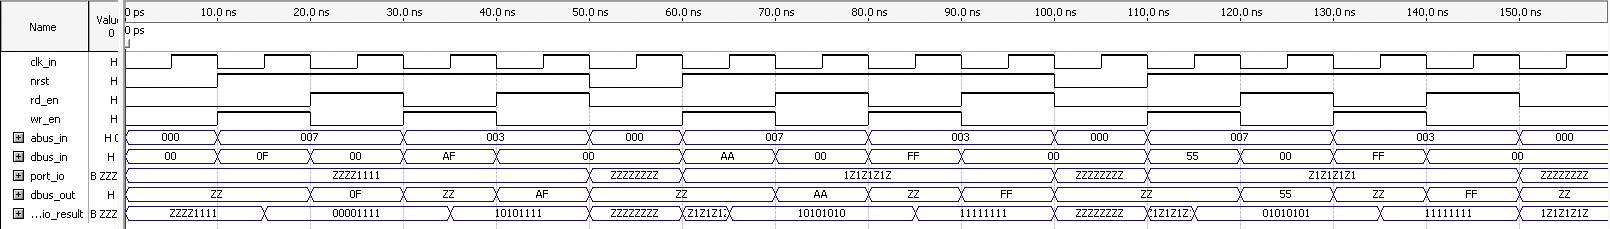
\includegraphics[width=15cm]{images/sim-port-io.png}
    \caption{Simulação do circuito port\_io}
\end{center}
\end{figure}

\newpage

\section{ram\_mem}

O bloco ram\_mem é um circuito que funciona como uma memória RAM. Ele é dividido em 4 blocos: 3 de 80 bytes, e 1 de 16 bytes. A escrita e leitura em cada um desses blocos é invisível para o usuário. Isto é, apenas um espaço de endereçamento é utilizado, e o circuito deve manejar em qual bloco escrever, ou ler, de acordo com a especificação.

\begin{table}[ht]
    \begin{center}
        \begin{tabular}{|c|c|c|c|}
            \hline
            Nome & Tamanho & Tipo & Descrição\\
            \hline
            nrst & 1 bit & \textit{Input} & Entrada de \textit{reset} assíncrono.\\
            \hline
            clk\_in & 1 bit & \textit{Input} & Entrada de \textit{clock}.\\
            \hline
            abus\_in & 9 bit & \textit{Input} & Entrada de enderençamento.\\
            \hline
            dbus\_in & 8 bits & \textit{Input} & Entrada de dados para escrita.\\
            \hline
            wr\_en & 1 bit & \textit{Input} & Entrada de habilitação de escrita.\\
            \hline
            rd\_en & 1 bit & \textit{Input} & Entrada de habilitação de leitura.\\
            \hline
            dbus\_out & 8 bits & \textit{Output} & Saída de dados hailitada por rd\_en.\\
            \hline
        \end{tabular}
    \end{center}
    \caption{Entradas e Saídas de ram\_mem}
\end{table}

\begin{table}[ht]
    \begin{center}
        \begin{tabular}{|c|c|}
            \hline
            Bloco & Faixa de endereçamento \\
            \hline
            mem0 & 020h $\sim$ 06Fh (80 bytes). Em decimal: 32 a 111 \\
            \hline
            mem1 & 0A0h $\sim$ 0EFh (80 bytes). Em decimal: 160 a 239 \\
            \hline
            mem2 & 20h $\sim$ 16Fh (80 bytes). Em decimal: 288 a 367 \\
            \hline
            mem\_com & 070h $\sim$ 07Fh (16 bytes). Em decimal: 112 a 127 \\
            \hline
        \end{tabular}
    \end{center}
    \caption{Entradas e Saídas de ram\_mem}
\end{table}

A área de memória mem\_com também pode ser endereçada através dos endereços 0F0h $\sim$ 0FFh,
170h $\sim$ 17Fh ou 1F0h $\sim$ 1FFh. Dessa forma os bits 8 e 7 de abus\_in não importam para o endereçamento
dessa área específica, sendo utilizados apenas os bits 6 a 0.

\subsection{Implementação}

O circuito ram\_mem foi implementado utilizando a linguagem VHDL.\\

O código na íntegra está abaixo:\\

\begin{lstlisting}[language=VHDL, caption={Código VHDL fsr\_reg}]
LIBRARY ieee;
USE ieee.std_logic_1164.all;
USE ieee.std_logic_unsigned.all;
USE ieee.numeric_std.all;

ENTITY ram_mem IS
    PORT (
        -- Inputs
        nrst : IN STD_LOGIC;                            -- Reset
        clk_in: IN STD_LOGIC;                           -- Clock
        abus_in: IN STD_LOGIC_VECTOR(8 DOWNTO 0);       -- Enderecamento
        dbus_in: IN STD_LOGIC_VECTOR(7 DOWNTO 0);       -- Dados
        wr_en : IN STD_LOGIC;                           -- Enable escrita
        rd_en : IN STD_LOGIC;                           -- Enable leitura

        -- Outputs
        dbus_out : OUT STD_LOGIC_VECTOR(7 DOWNTO 0)     -- Dados
    );
END ENTITY;

ARCHITECTURE ram_mem OF ram_mem IS
    TYPE mem_type0 IS ARRAY(0 TO 79) OF STD_LOGIC_VECTOR(7 DOWNTO 0);
    TYPE mem_type1 IS ARRAY(0 TO 15) OF STD_LOGIC_VECTOR(7 DOWNTO 0);

    SIGNAL mem0: mem_type0;
    SIGNAL mem1: mem_type0;
    SIGNAL mem2: mem_type0;
    SIGNAL mem_com: mem_type1;
    SIGNAL addr_int : INTEGER RANGE 0 TO 511;

BEGIN
    addr_int <= TO_INTEGER(UNSIGNED(abus_in));

    PROCESS(clk_in, nrst, addr_int, rd_en)
    BEGIN
        IF RISING_EDGE(clk_in) THEN
            IF wr_en = '1' THEN
                CASE addr_int IS 
                    -- mem0 80 bytes
                    WHEN 32 TO 111 =>
                        mem0(addr_int - 32) <= dbus_in;

                    -- mem1 80 bytes
                    WHEN 160 TO 239 =>
                        mem1(addr_int - 160) <= dbus_in;

                    -- mem2 80 bytes
                    WHEN 288 TO 367 =>
                        mem2(addr_int - 288) <= dbus_in;

                    -- mem_com 16 bytes
                    WHEN 112 TO 127 =>
                        mem_com(addr_int - 112) <= dbus_in;
                    WHEN 240 TO 255 =>
                        mem_com(addr_int - 240) <= dbus_in;
                    WHEN 368 TO 383 =>
                        mem_com(addr_int - 368) <= dbus_in;
                    WHEN 496 TO 511 =>
                        mem_com(addr_int - 496) <= dbus_in;

                    -- default
                    WHEN OTHERS =>
                END CASE;
            END IF;

        END IF;
        
        IF nrst = '0' THEN
            mem0 <= (OTHERS => (OTHERS => '0'));
            mem1 <= (OTHERS => (OTHERS => '0'));
            mem2 <= (OTHERS => (OTHERS => '0'));
            mem_com <= (OTHERS => (OTHERS => '0'));
        END IF;
    END PROCESS;

    PROCESS(clk_in, addr_int, rd_en, mem0, mem1, mem2, mem_com)
    BEGIN
        IF rd_en = '1' THEN
            CASE addr_int IS 
                -- mem0 80 bytes
                WHEN 32 TO 111 =>
                    dbus_out <= mem0(addr_int - 32);

                -- mem1 80 bytes
                WHEN 160 TO 239 =>
                    dbus_out <= mem1(addr_int - 160);

                -- mem2 80 bytes
                WHEN 288 TO 367 =>
                    dbus_out <= mem2(addr_int - 288);

                -- mem_com 16 bytes
                WHEN 112 TO 127 =>
                    dbus_out <= mem_com(addr_int - 112);
                WHEN 240 TO 255 =>
                    dbus_out <= mem_com(addr_int - 240);
                WHEN 368 TO 383 =>
                    dbus_out <= mem_com(addr_int - 368);
                WHEN 496 TO 511 =>
                    dbus_out <= mem_com(addr_int - 496);

                -- default
                WHEN OTHERS =>
            END CASE;
        ELSE
            dbus_out <= "ZZZZZZZZ";
        END IF;
    END PROCESS;
END ram_mem;     
\end{lstlisting}

\subsubsection{Descrição do funcionamento}

O circuito implementado possui duas partes: uma síncrona e outra assíncrona. A leitura é feita de forma síncrona, isto é, junto de uma borda de subida do \textit{clock}, já a leitura é feita de forma assíncrona.

Primeiramente, se converte o sinal de entrada abus\_in para um inteiro, utilizando a função \textit{TO\_INTEGER()}. Com isso, podemos identificar se o endereço sendo lido/escrito está dentro dos intervalos identificados.

Dentro da seção síncrona, após uma borda de subida de \textit{clock}, os dados são escritos no bloco correto, caso rd\_en esteja ativo. Já na parte assíncrona, caso wr\_en esteja ativo, o valor endereçado é colocado na saída, acessado de acordo com o bloco utilizado.

O \textit{reset} é feito de maneira assíncrona, e possui preferência sobre a escrita, pois é feita de maneira procedural, após ela.

\subsection{Simulação}

Para testar nosso código VHDL e certificar-nos de que nosso circuito funciona de maneira esperada, simulamos alguns casos de testes utilizando o software Quartus II.\\

Os testes realizados foram os seguites:

\begin{figure}[ht]
\begin{center}
        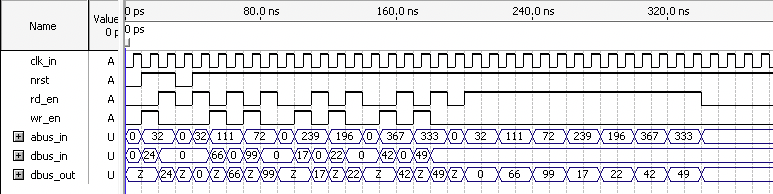
\includegraphics[width=15cm]{images/ram-mem-all.png}
        \caption{Simulação realizada com todos os blocos em conjunto.}
\end{center}
\end{figure}

\subsubsection{Registrador mem0}

\begin{enumerate}
    \item  Escrita e leitura com menor endereço possível.
    \begin{itemize}
        \item abus\_in = 32;
        \item dbus\_in = 24;
        \item \textbf{Comportamento esperado:}
        \begin{itemize}
            \item dbus\_out = 24;
        \end{itemize}
    \end{itemize}
    
    \item Testa leitura após reset.
    \begin{itemize}
        \item abus\_in = 32;
        \item dbus\_in = 0;
        \item \textbf{Comportamento esperado:}
        \begin{itemize}
            \item dbus\_out = 0;
        \end{itemize}
    \end{itemize}

    \item  Escrita e leitura com maior endereço possível.
    \begin{itemize}
        \item abus\_in = 111;
        \item dbus\_in = 66;
        \item \textbf{Comportamento esperado:}
        \begin{itemize}
            \item dbus\_out = 66;
        \end{itemize}
    \end{itemize}

    \item  Escrita e leitura com endereço aleatório.
    \begin{itemize}
        \item abus\_in = 72;
        \item dbus\_in = 99;
        \item \textbf{Comportamento esperado:}
        \begin{itemize}
            \item dbus\_out = 99;
        \end{itemize}
    \end{itemize}
\end{enumerate}

\begin{figure}[ht]
    \begin{center}
        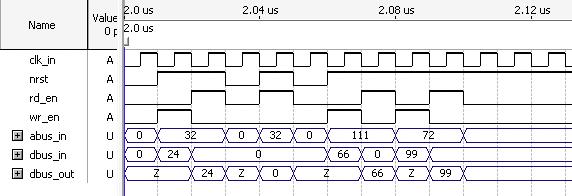
\includegraphics[width=15cm]{images/ram-mem0.png}
        \caption{Simulação mem0}
\end{center}
\end{figure}

\subsubsection{Registrador mem1}

\begin{enumerate}
    \item  Escrita e leitura com menor endereço possível.
    \begin{itemize}
        \item abus\_in = 160;
        \item dbus\_in = 13;
        \item \textbf{Comportamento esperado:}
        \begin{itemize}
            \item dbus\_out = 13;
        \end{itemize}
    \end{itemize}
    
    \item Testa leitura após reset.
    \begin{itemize}
        \item abus\_in = 160;
        \item dbus\_in = 0;
        \item \textbf{Comportamento esperado:}
        \begin{itemize}
            \item dbus\_out = 0;
        \end{itemize}
    \end{itemize}

    \item  Escrita e leitura com maior endereço possível.
    \begin{itemize}
        \item abus\_in = 239;
        \item dbus\_in = 17;
        \item \textbf{Comportamento esperado:}
        \begin{itemize}
            \item dbus\_out = 17;
        \end{itemize}
    \end{itemize}

    \item  Escrita e leitura com endereço aleatório.
    \begin{itemize}
        \item abus\_in = 196;
        \item dbus\_in = 22;
        \item \textbf{Comportamento esperado:}
        \begin{itemize}
            \item dbus\_out = 22;
        \end{itemize}
    \end{itemize}
\end{enumerate}

\begin{figure}[ht]
    \begin{center}
            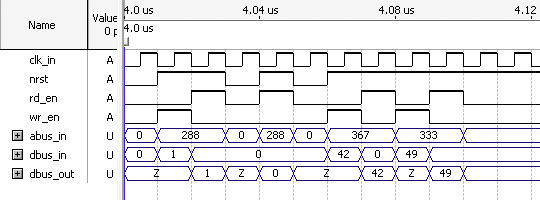
\includegraphics[width=15cm]{images/ram-mem1.png}
            \caption{Simulação mem1}
    \end{center}
    \end{figure}

\subsubsection{Registrador mem2}

\begin{enumerate}
    \item  Escrita e leitura com menor endereço possível.
    \begin{itemize}
        \item abus\_in = 288;
        \item dbus\_in = 1;
        \item \textbf{Comportamento esperado:}
        \begin{itemize}
            \item dbus\_out = 1;
        \end{itemize}
    \end{itemize}
    
    \item Testa leitura após reset.
    \begin{itemize}
        \item abus\_in = 288;
        \item dbus\_in = 0;
        \item \textbf{Comportamento esperado:}
        \begin{itemize}
            \item dbus\_out = 0;
        \end{itemize}
    \end{itemize}

    \item  Escrita e leitura com maior endereço possível.
    \begin{itemize}
        \item abus\_in = 367;
        \item dbus\_in = 17;
        \item \textbf{Comportamento esperado:}
        \begin{itemize}
            \item dbus\_out = 17;
        \end{itemize}
    \end{itemize}

    \item  Escrita e leitura com endereço aleatório.
    \begin{itemize}
        \item abus\_in = 333;
        \item dbus\_in = 49;
        \item \textbf{Comportamento esperado:}
        \begin{itemize}
            \item dbus\_out = 49;
        \end{itemize}
    \end{itemize}
\end{enumerate}

\begin{figure}[ht]
\begin{center}
        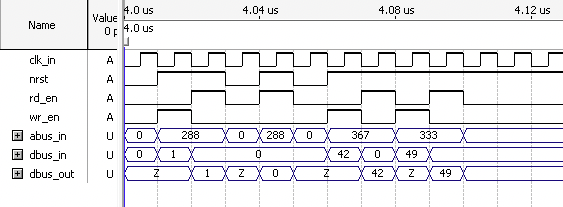
\includegraphics[width=15cm]{images/ram-mem2.png}
        \caption{Simulação mem2}
\end{center}
\end{figure}

\subsubsection{Registrador mem\_com}

\begin{enumerate}
    \item  Escrita e leitura com menor endereço possível.
    \begin{itemize}
        \item abus\_in = 112;
        \item dbus\_in = 24;
        \item \textbf{Comportamento esperado:}
        \begin{itemize}
            \item dbus\_out = 24;
        \end{itemize}
    \end{itemize}
    
    \item Testa leitura após reset.
    \begin{itemize}
        \item abus\_in = 112;
        \item dbus\_in = 0;
        \item \textbf{Comportamento esperado:}
        \begin{itemize}
            \item dbus\_out = 0;
        \end{itemize}
    \end{itemize}

    \item  Escrita e leitura com endereço 127.
    \begin{itemize}
        \item abus\_in = 127;
        \item dbus\_in = 66;
        \item \textbf{Comportamento esperado:}
        \begin{itemize}
            \item dbus\_out = 66;
        \end{itemize}
    \end{itemize}

    \item  Escrita e leitura com endereço 120.
    \begin{itemize}
        \item abus\_in = 120;
        \item dbus\_in = 100;
        \item \textbf{Comportamento esperado:}
        \begin{itemize}
            \item dbus\_out = 100;
        \end{itemize}
    \end{itemize}

    \item  Escrita e leitura com endereço 245.
    \begin{itemize}
        \item abus\_in = 245;
        \item dbus\_in = 37;
        \item \textbf{Comportamento esperado:}
        \begin{itemize}
            \item dbus\_out = 37;
        \end{itemize}
    \end{itemize}

    \item  Escrita e leitura com endereço 370.
    \begin{itemize}
        \item abus\_in = 370;
        \item dbus\_in = 123;
        \item \textbf{Comportamento esperado:}
        \begin{itemize}
            \item dbus\_out = 123;
        \end{itemize}
    \end{itemize}

    \item  Escrita e leitura com endereço 500.
    \begin{itemize}
        \item abus\_in = 500;
        \item dbus\_in = 8;
        \item \textbf{Comportamento esperado:}
        \begin{itemize}
            \item dbus\_out = 8;
        \end{itemize}
    \end{itemize}
\end{enumerate}

\begin{figure}[ht]
\begin{center}
    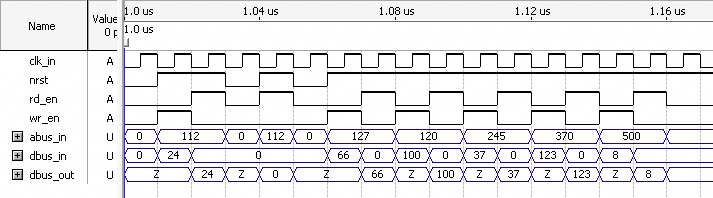
\includegraphics[width=15cm]{images/ram-mem-com.png}
    \caption{Simulação mem\_com}
\end{center}
\end{figure}

\section{Conclusão}

Neste trabalho trabalho prático, tivemos a oportunidade de desenvolver dois circuitos importantes para funcionamento de um processador.

O port\_io tange o interfaceamento entre o processador e o mundo externo, já o ram\_mem é a estrutrura responsável por armazenar dados e instruções que usadas pelo processador (como nossos programas).

\end{document}